\documentclass[spanish,notitlepage,letterpaper,11pt]{article} % para artÌculo en castellano
\usepackage[utf8]{inputenc} % Acepta caracteres en castellano
\usepackage[T1]{fontenc} % font encoding
\usepackage[spanish]{babel}    % silabea palabras castellanas
\usepackage[none]{hyphenat} 
\usepackage{amsmath}
\usepackage{amsfonts}
\usepackage{amssymb}
\usepackage[colorlinks=true,urlcolor=blue,linkcolor=blue]{hyperref} % navega por el doc
\usepackage{graphicx}
\usepackage{geometry}      % See geometry.pdf to learn the layout options.
\geometry{letterpaper}       
\usepackage{mathrsfs}% ... or a4paper or a5paper or ... 
%\geometry{landscape}                % Activate for for rotated page geometry
%\usepackage[parfill]{parskip}    % Activate to begin paragraphs with an empty line rather than an indent
\usepackage{epstopdf}
\usepackage{fancyhdr} % encabezados y pies de pg
\usepackage{lineno}
%\linenumbers

\pagestyle{fancy} 
\chead{\bfseries Lectures on special relativity} 
\lhead{} % si se omite coloca el nombre de la seccion
\rhead{25/05/2020} 
\lfoot{\it Miguel Jafert Serrano Mantilla } 
\cfoot{Universidad Industrial de Santander} 
\rfoot{\thepage} \documentclass[spanish,notitlepage,letterpaper,11pt]{article} % para artÌculo en castellano
\usepackage[utf8]{inputenc} % Acepta caracteres en castellano
\usepackage[T1]{fontenc} % font encoding
\usepackage[spanish]{babel}    % silabea palabras castellanas
\usepackage[none]{hyphenat} 
\usepackage{amsmath}
\usepackage{amsfonts}
\usepackage{amssymb}
\usepackage[colorlinks=true,urlcolor=blue,linkcolor=blue]{hyperref} % navega por el doc
\usepackage{graphicx}
\usepackage{geometry}      % See geometry.pdf to learn the layout options.
\geometry{letterpaper}                   % ... or a4paper or a5paper or ... 
%\geometry{landscape}                % Activate for for rotated page geometry
%\usepackage[parfill]{parskip}    % Activate to begin paragraphs with an empty line rather than an indent
\usepackage{epstopdf}
\usepackage{fancyhdr} % encabezados y pies de pg
\usepackage{lineno}
%\linenumbers

\pagestyle{fancy} 
\chead{\bfseries LECTURES ON SPECIAL RELATIVITY} 
\lhead{} % si se omite coloca el nombre de la seccion
\rhead{22/10/2022} 
\lfoot{\it Jafert Serrano  } 
\cfoot{Universidad Industrial de Santander} 
\rfoot{\thepage} 

\voffset = -0.25in 
\textheight = 8.0in 
\textwidth = 6.5in
\oddsidemargin = 0.in
\headheight = 20pt 
\headwidth = 6.5in
\renewcommand{\headrulewidth}{0.5pt}
\renewcommand{\footrulewidth}{0,5pt}
\DeclareGraphicsRule{.tif}{png}{.png}{`convert #1 `dirname #1`/`basename #1 .tif`.png}

\begin{document}
\title{ LECTURES ON SPECIAL RELATIVITY}
\author{
\textbf{Miguel Jafert Serrano Mantilla } \\ 
\textit{Universidad Industrial de santander} \\ }
\date{Versión $1$ 22/10/2022 }
\maketitle
\tableofcontents
\begin{abstract}
I have got recompiled in this document all the material and physical reasoning about the mathematical tools of the special relativity trying to be specific but keeping it simple, what I'm trying to say is that all the mathematic used in here is gonna be interpreted as simple as I can.

\end{abstract}
\section{Historical context}


\section{Postulates}

The special relativity has got a strong mathematical formation thus it must have some postulates which we can construct this theory, such postulates are the following:

\begin{enumerate}
    \item The inertial systems are characterized by the following properties: 
    
    \begin{itemize}
        \item The free particles move in straight trajectories. 
        \item The speed of light is independent of the inertial system.
    \end{itemize}
    
    \item The mechanic's and electromagnetism's laws are the same for every inertial system. 
\end{enumerate}

With these two postulates is enough to create a solid theory for the special relativity. From now on the star of the show is what we call the events space , a fourth-dimensional space where exist all the motion events in any point of the space-time.

\subsection{Light cone}\label{sc: LC}

\begin{figure}[h]
    \centering
    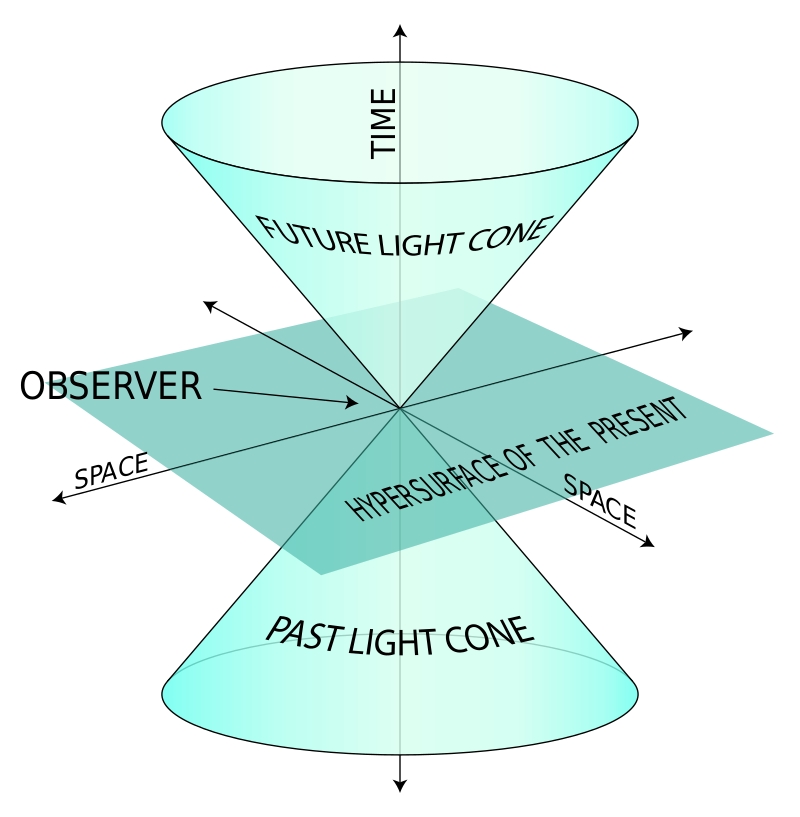
\includegraphics[width = 0.5\textwidth]{Images/LightCone.png}
    \caption{Light cone illustration. Imagen from: \cite{enwiki:1112919376}}
    \label{fig:LC1}
\end{figure}

The light cone is the region made by a light beam that starts at a given event $\mathscr{E} = (t,\vec{x})$ it's hard the first time see the importance of this cone, lets give a look to the figure \ref{fig:LC1} we see that the cone divides the space in two regions, in the top the cone encloses all the future events we are going to be able to live, all the adventures we as observers are going to experience, and below in that past light cone rest all the things we've already lived and learned. No matter how beauty this sounds, but is beauty, this interpretations depends on one signs convention we must discuss and adopt one or the other a bit latter, what a I mean is that all what I just said depends if we're inside or outside the cone but latter with the signs convention we will choose being out or in the cone.\\


The past or future is independent from the reference system, so this cone must not dependt on the coodinate syste, thus in every event there is a light cone, shuch that: $\mathscr{E} = (t , \vec{x}$) or:

\begin{equation}\label{eq::LCE}
    C_{\mathscr{E}} := \{(s,\vec{x}) \in \mathbb{R}^4 :C|s-t| = |\vec{y} - \vec{x}| \}
\end{equation}

Is easily to see the equation \ref{eq::LCE} es a cone equation, so let $\mathcal{L}$ a transformation between inertial systems, thus:

\begin{equation*}
    \mathcal{L}(\mathscr{E}) = \mathscr{E}' \rightarrow \mathcal{L}(C_{\mathscr{E'}}) = C_{\mathscr{E}}
\end{equation*}

\begin{equation*}
    (t,\vec{x}) \rightarrow (t',\vec{x}') 
\end{equation*}

These two transforms make the Poincaré's group and inside this group there is the Lorent'z group.

\subsection{Poincaré's transforms}
\subsubsection{Recordatorio}
PENDINTE MMMM

\section{Minkowski's space-time}

The German scientific Hermann Minkowski postulated this space where we can construct the special relativity, we call the $\textit{Minkoski's space-time}$ to a vectorial space ,where the speed of light $C$ is equal to $1$, that's called \textit{natural coordinates} or \textit{geometrized coordinates}, of the form:

\begin{equation*}
    \xi = (\mathbb{R}^4, <\cdot,\cdot>)
\end{equation*}

This means our space is made by our well known $\mathbb{R}^4$ space, and a Lorentzian inner product, whi is a pseudo- Reinmannian inner product. Let $\vec{V} , \vec{W}  \in \;\;\mathbb{R}^4$ then the inner product is:

\begin{equation}\label{eq:IP}
    <\vec{V},\vec{W}> = -V^0W^0 + V^1W^1 + V^2W^2 + V^3W^3
\end{equation}

The equation \ref{eq:IP} can be written in a more compact form using a tensorial formalism like this:

\begin{equation}\label{eq:IPT}
    <\vec{V},\vec{W}> = \eta_{\alpha\beta}V^{\alpha}W^{\beta}
\end{equation}

where:

\begin{equation}\label{eq:metric}
    [\eta_{\alpha\beta}] = 
    \begin{bmatrix}
    -1 & 0 & 0 & 0 \\
    0 & 1 & 0 & 0 \\
    0 & 0 & 1 & 0 \\
    0 & 0 & 0 & 1
    \end{bmatrix}
\end{equation}

Here there are a lot of things to discuss, the first thing that rises is that the equation \ref{eq:IPT} doesn't define a Reinmannian inner product, because it is not always positive-defined that's the reason for calling it \textit{pseudo-Reinmannian inner product} now it's time to remind the 
discussion started in \ref{sc: LC} where we didn't know exactly in what point we live, to answer that lets give a look to the equation \ref{eq:metric} which is the metric of our space-time, this is no the only way to write the metric, this is using the \textbf{mostly positive} signature or $(-,+,+,+)$ signature, there's another one the \textbf{mostly negative signature} or $(+,+,+,-)$ signature .\\

If the equation \ref{eq:IP} is equal to $0$ we've got a cone equation! and if we give a look no matter what signature we choose is the same cone, but the interpretation of our position respect to the cone varies slightly , if the choose the mostly positive signature and our spatial part is less or equal than the temporal part that means we are always inside the cone or in the surface, respectively , if we choose the mostly negative signature the interpretation is the other way around, but the interpretation of the space-time evolution is the same. All the equations obtained by one or the other signature are completely isomorphic, here we choose the mostly positive signature. Now lets give a look to the distances:

\begin{equation*}
    \eta_{\alpha\beta}\triangle x^{\alpha}\triangle x^{\beta} = -\triangle t^2 + |\vec{x}|^2 = 0 \;\; : \;\; \triangle x^{\alpha} = X_2^{\alpha} - x_1^{\alpha}
\end{equation*}

This should look simple but it is really important for us, because we are saying that the distance between events doesn't depend on the system, the measure of distance must not depend of the coordinate system and if we give a look, the last equation also describes a cone, amazing! the cone equation also keeps invariant, our space-time evolution is intact. \textbf{Remark:} Is we don't use natural coordinates the equation varies a bit, a $C^2$ appears in the time side of the equation.

\subsection{Affine transformation}

All the transformations in our space-time at this moment are affine transformations , transform made by one linear transformation plus a displacement , in the Newtonian case we've got the Galileo's Group which has the form:

\begin{equation}\label{eq:GalieoG}
    T_\mathscr{G}(\vec{x}) = \hat{G}\vec{x} + \vec{v}t \;\; : \;\; \{\vec{x},\vec{v} \in \mathbb{R}^3\} \;\; t \in \mathbb{R}
\end{equation}

The equation \ref{eq:GalieoG} is a compact form of writting the elements of the Galileo's group $\mathscr{G} = (S , °)$ with the elements $S$ :

\begin{enumerate}
    \item Uniform motion with velocity $\vec{v}$:
    \begin{equation*}
        s_1(t,\vec{x}) = (t , \vec{x} + \vec{v}t) \;\; \forall t \in \mathbb{R}^3 \;,\; \vec{x} \in \mathbb{R}^3
    \end{equation*}
    
    \item Translation of the origin:
    \begin{equation*}
        s_2(t,\vec{x}) = (t + s , \vec{x} + \vec{w}) \;\; \forall t \in \mathbb{R}^3 \;,\; \vec{x} \in \mathbb{R}^3
    \end{equation*}
    
    \item Rotation of the coordinate axes:
    \begin{equation*}
        s_3(t,\vec{x}) = (t , \hat{R}\vec{x} ) \;\; \forall t \in \mathbb{R}^3 \;,\; \vec{x} \in \mathbb{R}^3
    \end{equation*}
    
    Where $\hat{R}: \mathbb{R}^3 \rightarrow \mathbb{R}^3$ is an orthogonal transformation.
\end{enumerate}

In the same way we're gonna deduce the affine transform for Minkowskian space-time, let $\vec{x}'$ a vector which obeys an affine transformation as:

\begin{equation*}
    \vec{x}' = \mathcal{L}(\vec{x}) = \Lambda \vec{x} + \vec{a} \;\; :\;\; \vec{x},\vec{a}\in \mathbb{R}^4 \;\;, \;\; \Lambda \in G_L,
\end{equation*}

Where $G_L$ is the Lorentz's group, but before doing that, lets discover the linear transform case:

\begin{equation}\label{eq:LT}
    \vec{x}' = \Lambda \vec{x}
\end{equation}

The transform $\Lambda$ must give invariant the light cone so let $\vec{v} , \vec{w} \in \mathbb{R}^4$:

\begin{equation*}
    <\Lambda \vec{v} , \Lambda \vec{w} > = <\vec{v} , \vec{w}> \rightarrow (\Lambda \vec{v})^T\eta(\lambda\vec{w}) = \vec{v}^T \eta \vec{w}
\end{equation*}

\begin{equation*}
    \vec{v}^T\Lambda^T\eta\Lambda\vec{w} = \vec{v}^T\eta\vec{w}
\end{equation*}

\begin{equation}\label{eq:eta}
    \eta = \Lambda ^T \eta \Lambda
\end{equation}

The equation \ref{eq:eta} is a similarity transform, is easily to see that $\Lambda$ only could have two values for its determinant $|\Lambda| = \pm 1$. \\

Demonstration:

\begin{equation}\label{eq:deteta}
    |\eta| = |\Lambda^T\eta\Lambda| = |\Lambda^T|*|\eta|*|\Lambda|,
\end{equation}

We can see in \ref{eq:metric} that $|\eta| = -1$ and using the properties $|A| = |A^T|$ we can rewrite the equation \ref{eq:deteta} as:

\begin{equation*}
    1 = |\Lambda|^2 \rightarrow |\Lambda| = \pm 1.
\end{equation*}

This is only possible in three cases:

\begin{enumerate}
    \item Temporal or parity inversions:
    \begin{equation*}
        \Lambda = diag[\mp 1 , \pm 1 , \pm 1 , \pm 1]
    \end{equation*}
    Respectively
    
    \item Unitary transformations:
    \begin{equation*}
        \Lambda = 
        \begin{bmatrix}
        1 & \vec{
        \mathcal{O}}^T \\
        \vec{\mathcal{O}} & R
        \end{bmatrix} \;\; : \;\; R \in SO(3)
    \end{equation*}
    
    \item Speed boots, for example a x boost:
    \begin{equation}
        \Lambda = 
        \begin{bmatrix}
        \gamma & -v_x\gamma & 0 & 0\\
        -v_x\gamma & \gamma & 0 & 0\\
        0 & 0 & 1 & 0\\
        0 & 0 & 0 & 1\\
        \end{bmatrix} \;\; : \gamma = \frac{1}{\sqrt{1 - v_x^2}} \;&\; C = 1
    \end{equation}
    If we are out from the natural coordinates $\gamma$ changes to $\gamma = \frac{1}{\sqrt{1 - \frac{v^2}{C^2}}}$
\end{enumerate}

As the Galilean group the Lorentz's group is made by $6$ elements, $3$ rotations and $3$ speed boosts, but in general:

\begin{equation*}
    \mathcal{L}(\vec{x}) = \Lambda \vec{x} + \vec{a} \;\;:\;\; \vec{x},\vec{a} \in \mathbb{R}^4
\end{equation*}

That general form is more general than the last one, we obtain it from de Lorentz's group $G_L$ and $4$ translations , we call it the \textit{Poincaré's group} $G_{\mathscr{P}}$.


\section{Lorentz transformations}

Let $\mathcal{O} \wedge \Bar{\mathcal{O}}$ intertial observers such that there is a relative movement between them, thus: $\Bar{\mathcal{O}} \rightarrow v \;\; : v < 1$ relative to $\mathcal{O} \wedge v > 1$ in the $x$  direction, thus the coordinates transformated are:

\begin{align*}
    \Bar{t} = At + Bx \\
    \Bar{x} = Ct + Dx \\
    \Bar{y} = y\\
    \Bar{z} = z
\end{align*}

Now, because the light cone is invariant we've got the following equation:

\begin{align*}
    -t^2 + x^2 + y^2 + z^2 = -\Bar{t}^2 + \Bar{x}^2 + \Bar{y}^2 + \Bar{z}^2 \\
    -t^2 + x^2 = -(A^2 - C^2)t^2 + (D^2-B^2)x^2 + 2(CD - AB)tx
\end{align*}

\begin{align*}
    A^2 - C^2 = 1\\
    D^2-B^2 = 1\\
    AB = CD\\
\end{align*}

This is a inconsistent system of equations, we've only 3 equations and fourth variables! But there're some special function that satisfies that equations, look at this equation: $cosh^2(\phi) - sinh^2(\phi) = 1$ THAT'S IT! There is our solution, thus: 

\begin{align*}
    A = D = cosh(\phi)\\
    C=B=-sinh(\phi)
\end{align*}

Thus our Lorentz's transformation becomes:

\begin{equation}
    \begin{bmatrix}
    \Bar{t}\\
    \Bar{x}
    \end{bmatrix}
    =
    \begin{bmatrix}
    cosh(\phi) & -sinh(\phi)\\
    -sinh(\phi) & cosh(\phi)
    \end{bmatrix}
    \begin{bmatrix}
    t\\
    x
    \end{bmatrix}
\end{equation}

That is a beautiful solution! Looks like a rotation! But it is not a rotation, we don't even know what in the hell is $\phi$ so lets find out what is $\phi$.\\

Let $\Bar{x} = 0$ thus $0 = -tsinh(\phi) + vtcosh(\phi)$ solving for $v$ we've got:

\begin{equation*}
    v = tanh(\phi) \rightarrow tanh^2(\phi)+ sech^2(\phi) = 1 \rightarrow sech(\phi) = \sqrt{1 - v^2}
\end{equation*}

\begin{align}
    \gamma = cosh(\phi) = \frac{1}{\sqrt{1 - v^2}}\\
    senh(\phi) = \frac{v}{\sqrt{1 - v^2}} = \gamma v
\end{align}

With all of this, we can get the final form of our Lorentz's tranformation:

\begin{align*}
    \Bar{t} = \gamma(t-vx)\\
    \Bar{x} = \gamma(x-vt)\\
    \Bar{y} = y\\
    \Bar{z} = z
\end{align*}

If we are not in natural coordinates, the transformation look like this:

\begin{align*}
    \Bar{t} = \gamma(t-\frac{v}{c^2}x)\\
    \Bar{x} = \gamma(x-vt)\\
    \Bar{y} = y\\
    \Bar{z} = z
\end{align*}

That is something really beautiful, only with the postulates easily we can get nature of the mechanics for high speeds, and easily see that the nature again follows a group's structure! Having all on count we can get the Lorentz's transform:

\begin{equation}\label{eq:GLT}
    [\Lambda] =
    \begin{bmatrix}
    \gamma & -\gamma v_x & -\gamma v_y & -\gamma v_z\\
    -\gamma v_x & 1+(\gamma - 1)\frac{v_x^2}{v^2} & (\gamma - 1)\frac{v_xv_y}{v^2} & (\gamma-1)\frac{v_xv_z}{v^2}\\
    -\gamma v_y & (\gamma - 1)\frac{v_yv_x}{v^2} & 1 + (\gamma - 1)\frac{v_y^2}{v^2} & (\gamma-1)\frac{v_yv_z}{v^2}\\
    -\gamma v_z & (\gamma-1)\frac{v_xv_z}{v^2} & (\gamma-1)\frac{v_yv_z}{v^2} & 1 +(\gamma - 1)\frac{v_z^2}{v^2}
    \end{bmatrix}
\end{equation}

The last equation is the most general Lorentz's transformation of the form: $\Bar{\vec{x}} = \Lambda(v)\vec{x}$

And our coordinate system transforms as follows:

\begin{figure}[h]
    \centering
    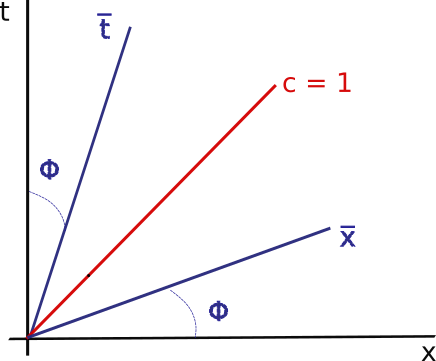
\includegraphics[width=0.5\textwidth]{Images/LorentzTransform_Layer 1.png}
    \caption{Invariance of the light cone under Lorentz's transfor}
    \label{fig:LCInvariance}
\end{figure}

\subsection{Recordatorio}
\textbf{Demonstration:} LA TENGO PENDIENTE

\subsection{Law of composition of speeds}

Here the composition of speeds isn't as easy as we've been working in the classical mechanics, so, let a particle with speed: $W = \frac{\triangle x}{\triangle t}$ respecto to $\mathcal{O}$ and $\Bar{W} = \frac{\Bar{\triangle x}}{\Bar{\triangle t}}$ respecto to $\Bar{\mathcal{O}}$ and using the Lorentz's transforms:

\begin{align*}
    \triangle\Bar{x} = \gamma(\triangle x - v\triangle t)\\
    \triangle\Bar{t} = \gamma(\triangle t - v\triangle x)
\end{align*}

Thus the speed of the particle respect to $\Bar{\mathcal{O}}$ is:

\begin{equation}
    \Bar{w} = \frac{w-v}{1-vw}
\end{equation}

Now, this is completely different respect to the Galilean composition of speeds, so is worthfull to analyze some cases:

\begin{enumerate}
    \item If the relative speed of the reference system is less than $1$ and the particle's speed respect to $\mathcal{O}$ is less than $1$ then the speed respect to $\Bar{\mathcal{O}}$ is less than 1. Demonstration: 
    
    \begin{itemize}
        \item
        \begin{align*}
            |w|<1 \rightarrow 1 + w > 0 \\
            |v|<1 \rightarrow v(1+w) < 1+w
        \end{align*}
        \begin{equation}\label{eq:IQ1}
        -(1-vw)> w-v
    \end{equation}
    
    \item
    \begin{align*}
        |w|<1 \rightarrow 1 + v>0 \\
        |w|<1 \rightarrow w(1+v) < 1 + v
    \end{align*}
    \begin{equation}\label{eq:IQ2}
        1-vw > w-v
    \end{equation}
    \end{itemize}
    
    The inequalities given in \ref{eq:IQ1} y \ref{eq:IQ2} are the definition of an absolute value, thus:
    \begin{equation*}
        |\Bar{w}| = \left|\frac{w-v}{1-vw}\right| < 1
    \end{equation*}
    
    \item If $w = 1$ then:
    \begin{equation*}
        \Bar{w} = \frac{1-v}{1-v} = 1
    \end{equation*}
    This means that the speed of light is independent of the coordinate system.
    
    \item If $v\ll1$ and $v\ll1$ then:
    \begin{equation*}
        \Bar{w} = w-v
    \end{equation*}
    That is the law of composition of speeds in the Galilean space!
    
    \item If $v=1$ thus the Lorentz's transforms are singular 
    \begin{figure}[h]
        \centering
        \includegraphics[width = 0.4\textwidth]{Images/Singular.png}
        \caption{Singularity of the Lorentz transform}
        \label{fig:SLT}
    \end{figure}
    
    \item If $|v| >1$ the Lorentz transforms are imaginary.
    
    \begin{figure}[h]
        \centering
        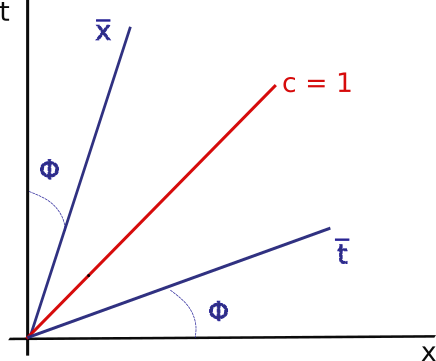
\includegraphics[width = 0.4\textwidth]{Images/Imaginary_Layer 1.png}
        \caption{Imaginary Lorentz transform}
        \label{fig:SLT}
    \end{figure}
    
    Here we see that the space-time is the other way around, instead of seeing a falling ball we see first the ball in the floor.
\end{enumerate}

\subsection{Proper time and the relativistic effects}

The space-time interval or the distant between events is invariant under Lorentz's transform, we define it as:

\begin{equation}\label{eq:IE}
    \triangle s^2 = <\triangle \vec{x} , \triangle \vec{x} > = \eta_{\alpha\beta}\triangle x^{\alpha}\triangle x^{\beta}
\end{equation}

\begin{equation*}
    \triangle\Bar{s}^2 = \triangle s^2
\end{equation*}

We can rewrite the equation \ref{eq:IE} as:

\begin{equation}
    \triangle s^2 = -\triangle t^2 \left[1 - \frac{\triangle x^2 + \triangle y^2 + \triangle z^2}{\triangle t^2}\right]
\end{equation}

We can rewrite it again as:
\begin{equation}
    -\triangle \tau^2 = -\triangle t^2(1-v^2) \rightarrow \triangle \tau = \frac{\triangle t}{\gamma}
\end{equation}

Where $\tau$ is the proper time, our "\textit{real}" time, and here we can see one of the effects of the special relativity, when you move, even more if it is a high speed, what you see is a time dilatation, that's because $\gamma \geq 1$ then $\triangle t \geq \triangle \tau$ , if we do an analogous calculus to \ref{eq:IE} we obtain a space contraction, when you see the bus escaping from you, you'll see that it is getting shorter when it accelerates and its time is going faster.
\section{Relativistic dynamics}

\subsection{Vectorial analysis in the special relativity}

\section{Differential Geometry }

\section{Relativistic electrodynamics}

Any event in the space-time can be describe with a vector like this: 

\begin{equation*}
    \vec{A} = [x_A^0,x_A^1,x_A^2,x_A^3]
\end{equation*}

And a displacement vector like:

\begin{equation*}
    \triangle\vec{x}= [\triangle x^0,\triangle x^1 , \triangle x^2 , \triangle x^3]
\end{equation*}

\begin{figure}[h]
    \centering
    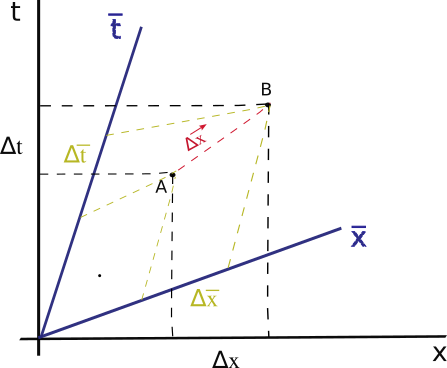
\includegraphics[width = 0.5\textwidth]{Images/Displacement_Layer 1.png}
    \caption{Relation between the transformed coordinates}
    \label{fig:my_label}
\end{figure}

The displacement should be independent of the coordinate system, so: $\triangle \vec{x} = [\triangle t, \triangle x ]_{\mathcal{O}} = [\triangle t, \triangle x ]_{\Bar{\mathcal{O}}}$ this for an one-dimensional movement

\section{Relativistic fluids}
 
\section{Lorentz's and Poincare's group}

\bibliographystyle{apalike}
\bibliography{Bibliografia.bib}

\end{document}  